\renewcommand{\proofname}{Доведення}
\renewcommand{\chaptername}{РОЗДІЛ}


\chapter{Тренди серед мобільних фреймворків}
\label{ch1}


\section{Розробка крос-платформних мобільних додатків}
\label{section.1.1}
Завдяки міжплатформенній розробці підприємства та організації змогли охопити ширшу аудиторію, ефективніше та з меншими витратами.
React Native був представлений Facebook у 2015 році.
React Native - це фреймворк для мобільних додатків з відкритим кодом, який використовує React із власними можливостями платформи для розробки додатків для Android, iOS, Web та UWP.

Серед рішень, що використовують React Native: Facebook, Instagram, Tesla, Uber Eats, Discord, Wix, Walmart.

Flutter був представлений Google у травні 2017 року. Але випуск стабільної версії відбувся у грудні 2018 року.
Flutter також має відкритий вихідний код і використовується для розробки програм для Android, iOS, Linux, Mac, Windows, Google Fuchsia та веб.

Деякі програми, створені за допомогою Flutter, це: Google Ads, Alibaba.com, Realtor.com.

Оскільки Flutter та React-Native стали найгарячішою темою останніх днів та конкурентними дебатами серед спільноти розробників, багато розробників залижаються у невизначеності, визначаючи, яку платформу вибрати.

Ідеальний розробник React Native повинен знати JavaScript + React Native SDK, Kotlin + Android SDK, Swift + iOS SDK, що в 3 рази більше знань у порівнянні зі звичайними розробниками мобільних пристроїв.
Звідси відсутність хороших розробників та підвищеня ціни (на щастя, не в 3 рази).
Як тільки ви вирішите використовувати React Native для свого проекту, не буде простого виходу.
Для переходу на інші кроссплатформенні фреймворки або власні мобільні програми потрібно буде повністю переписати.

Мова Dart була розроблена Google задовго до фреймворку, але вона намагалася знайти надійне прийняття.
Отже, всі розробники рівні з Flutter і їм потрібно навчитися з нуля.
Екосистема ще не настільки зріла, як реактивна, але швидко зростає.
Власні бібліотеки та код можна інтегрувати з програмами Flutter, тому потрібні також деякі навички iOS / Android.
Знову та сама проблема з 3 мовами, що вимагає від розробників одночасного володіння 3 технологіями.
Оскільки Flutter використовує Dart, а фреймворк написаний майже з нуля, розробникам буде важко перенести проекти Flutter на інші крос-платформні фреймворки або власні програми.
Буквально їм потрібно буде переписати все з нуля.

Цільова аудиторія Kotlin Multiplatform - це рідні розробники мобільних пристроїв, які вже використовують Kotlin на Android та Swift на iOS.
Іншими словами, це розробники, які глибоко розуміють рідні мобільні SDK, яким потрібно вивчити лише одну нову мову (Swift або Kotlin).
Таким чином, мультиплатформу Kotlin можна поступово вивчати за кілька тижнів.
Занадто добре, щоб бути правдою? Ну, є деякі недоліки, в основному пов’язані з тим, що Kotlin Multiplatform вийшов на Alpha лише кілька місяців тому.

\begin{center}
    \begin{longtable}{|p{0.23\textwidth}|p{0.22\textwidth}|p{0.22\textwidth}|p{0.23\textwidth}|}
        \caption{Порівняння Фреймворків}
        \label{tab:framwework_comparison}
        \\ \hline
        & React Native                               & Flutter                               & Kotlin Multiplatform                              \\
        \hline \endfirsthead
        \subcaption{Продовження таблиці~\ref{tab:framwework_comparison}}
        \\ \hline \endhead
        \hline \subcaption{Продовження на слід. стор.}
        \endfoot
        \hline \endlastfoot
        Вперше з’явився       & 2015                                & 2017                                & 2018                               \\
        \hline
        Розроблено                   & Facebook                         & Google                               & JetBrains                            \\
        \hline
        Відкрите джерело         & Так                                & Так                                & Так                               \\
        \hline
        Мова             & Javascript                           & Dart                           & Kotlin                               \\
        \hline
        Нативні Модулі & Так                      & Так                      & Так                             \\
        \hline
        Сумісність   & Обмежена & Обмежена & Так \\
        \hline
        Інші мови для вивчення                    & Kotlin, Swift                & Kotlin, Swift                     & Swift             \\
        \hline
        Клікість Розробників      & 42\%\cite{worldwide_sf_work_hours}                     & 39\%\cite{worldwide_sf_work_hours}                & 2\%\cite{worldwide_sf_work_hours}  \\
        \hline
        IDE      & Немає офіційної IDE                     & Android Studio                & Android Studio, XCode  \\
        \hline
        Цільова аудиторія      & Веб-розробники                     & Розробники флаттера                & Розробники під мобільні пристрої  \\
    \end{longtable}
\end{center}


\section{Тренди}\label{section.1.2}

\begin{figure}
    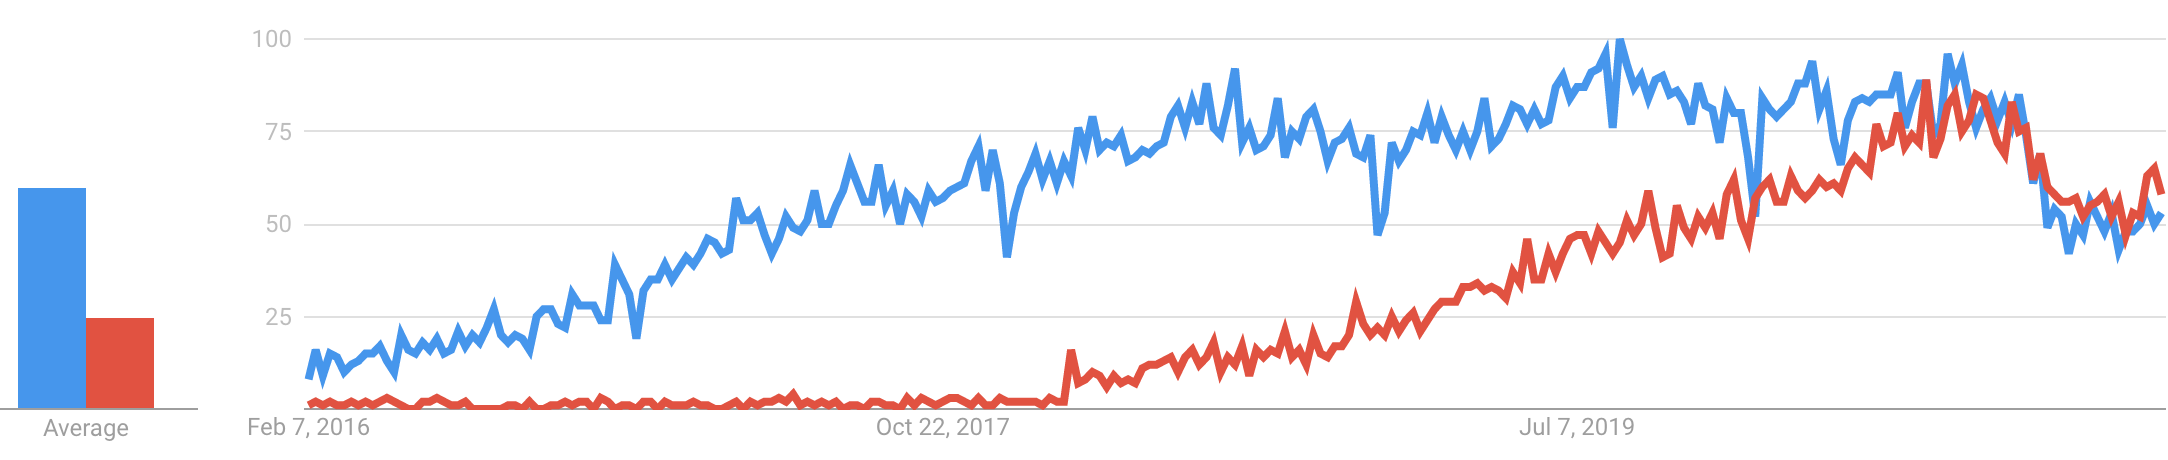
\includegraphics[width=\textwidth]{flutter_react_trend_5_years.png}
    \caption{Відповідно до Google Trends за 5 років}
    \label{fig:flutter_react_trend_5_years}
\end{figure}

На Google Trends за останні п’ять років Flutter випередив React Native див. мал.~\ref{fig:flutter_react_trend_5_years}.
Але це не визначає, що Flutter - кращий варіант, ніж React Native.

Порівнюючи тренди між Kotlin, Flutter та Reactive Native за 12 місяців також спостерігається більша зацікавленість Flutter.
Де Kotlin демонструє меньшу зацікавленість серед пошуків. див. мал.~\ref{fig:flutter_react_trend_12_months_1}.
\begin{figure}
    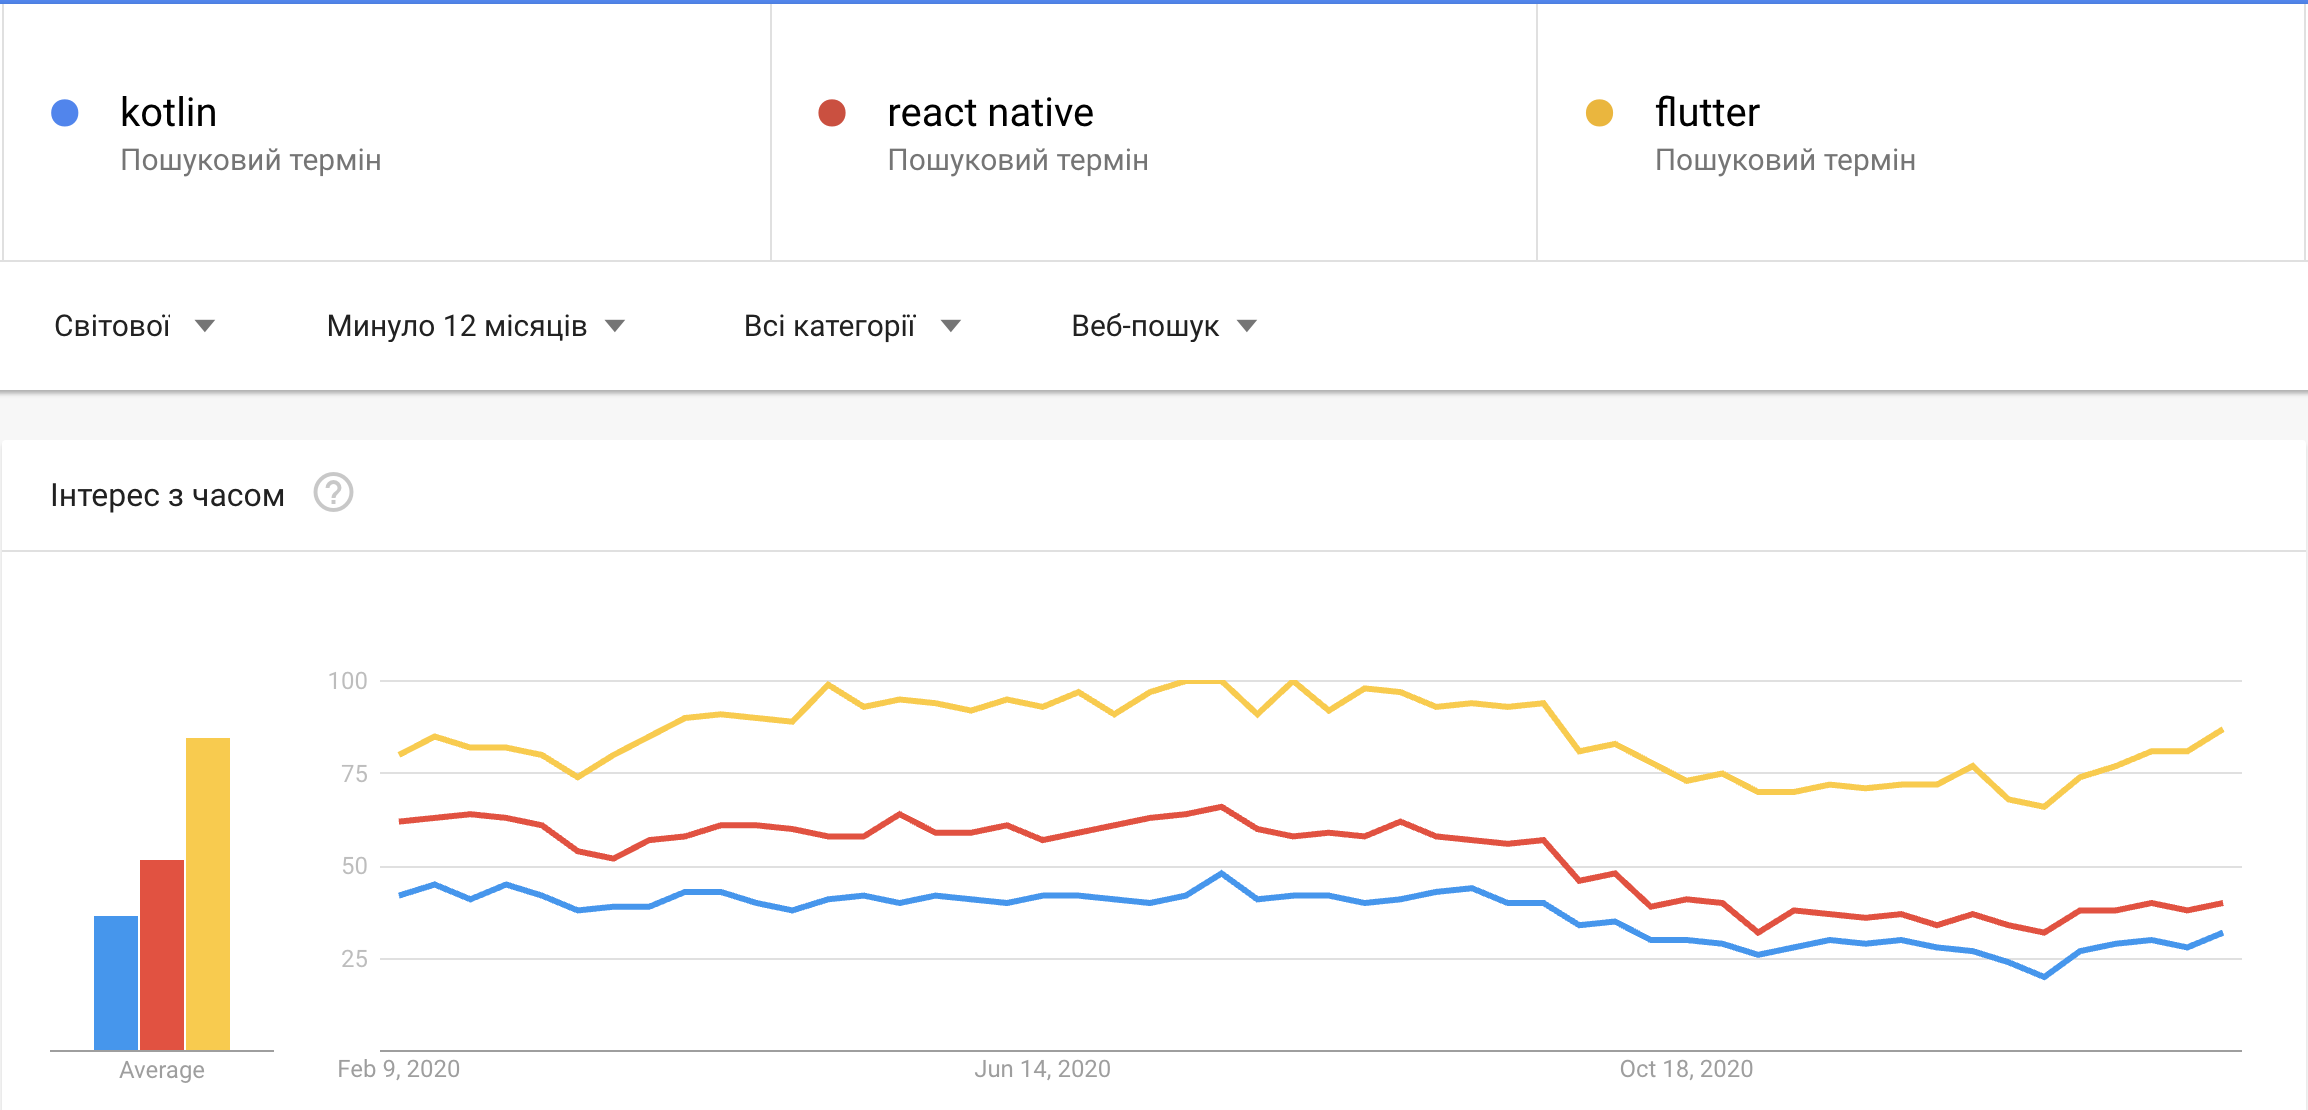
\includegraphics[width=\textwidth]{flutter_react_trend_12_months_1.png}
    \caption{Інтерес за часом Google Trends за 12 місяців \cite{google_trends}}
    \label{fig:flutter_react_trend_12_months_1}
\end{figure}

Оцінюючи мапу світу ми бачимо, що Flutter є лідером по зацікавленості сереж регіонів, коли React Native уступає всім трьом. див. мал.~\ref{fig:flutter_react_trend_12_months_2}.
\begin{figure}
    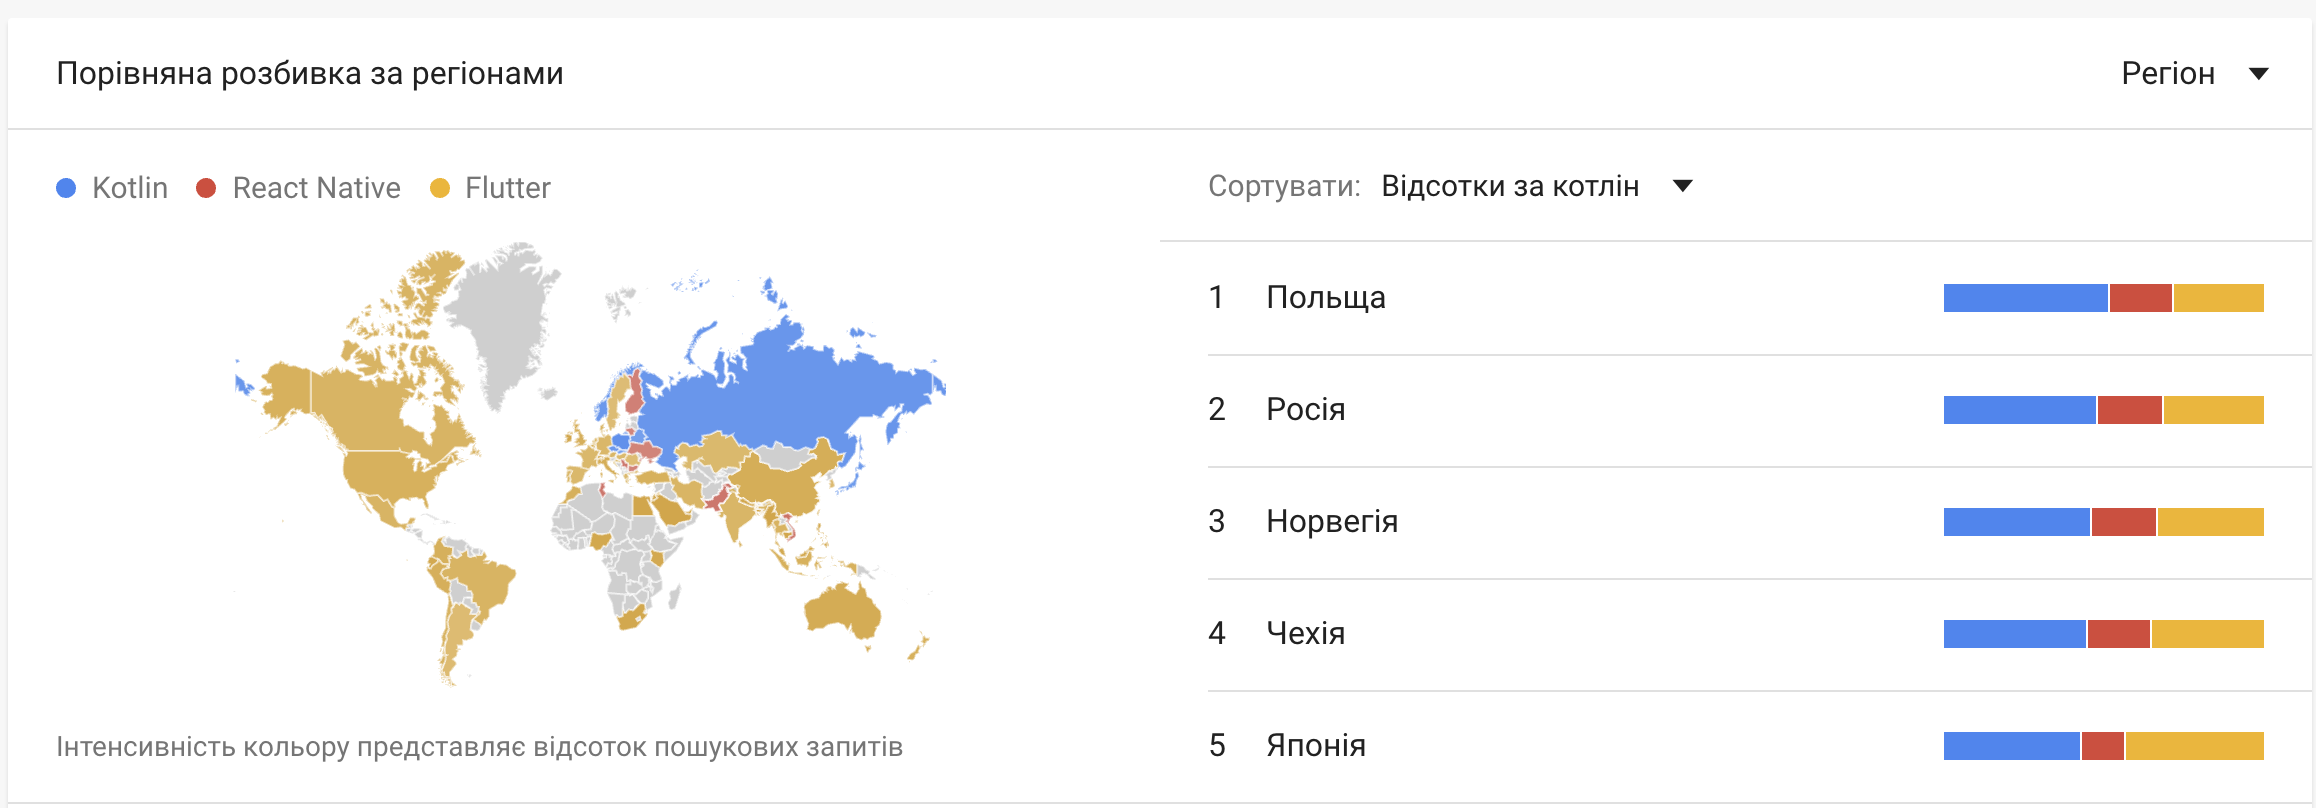
\includegraphics[width=\textwidth]{flutter_react_trend_12_months_2.png}
    \caption{Розбивка по регіонам \cite{google_trends}}
    \label{fig:flutter_react_trend_12_months_2}
\end{figure}

Що стосується міжплатформенних тенденцій розвитку технологій мобільних додатків, то і React Native, і Flutter досить схожі за популярністю, і обидва вони все ще досить молоді (React Native вийшов у 2015 році, Flutter у 2017 році).
Обидві технології посідають дуже високе місце на GitHub із 112 тис. зірок (Flutter) \cite{flutter_gihtub} та 93.2 тис. (React Native) \cite{rn_gihtub} за лютий 2021.

Ми бачимо, що інтерес до Флаттера значно зріс у 2021 році і швидко зростає.


\section{Переваги Flutter}\label{section.1.3}
\begin{enumerate}
    \begin{item}
        Одна кодова база.
        Flutter підтримує як мобільні платформи Android, так і iOS, і оскільки він відображає все самостійно, він дозволяє запускати все з однієї кодової бази.
        Це велика економія часу!
    \end{item}
    \begin{item}
        Красиві інтерфейси в найкоротші терміни.
        У Flutter користувальницький інтерфейс побудований за допомогою віджетів, невеликих будівельних блоків інтерфейсу, зібраних за допомогою техніки, що називається Композиція.
        Весь процес схожий на використання компонентів React.
        Існує два набори віджетів, що доступні нестандартно: Material Design, який сумісний з дизайнерськими вказівками Google, та Cupertino, сумісний з Apple's Interface Guidelines для iOS .
    \end{item}
    \begin{item}
        Візуалізація пікселів.
        Flutter управляє кожним пікселем екрану, тому ми можемо бути впевнені, що наші віджети будуть виглядати однаково на кожному мобільному пристрої (навіть на старих), по суті усуваючи наші потенційні проблеми з підтримкою пристрою.
        Це, в свою чергу, дозволяє нам створювати дивовижні на вигляд користувальницькі інтерфейси, які виглядають абсолютно однаково як на Android, так і на iOS з єдиною кодовою базою.
    \end{item}
    \begin{item}
        Швидша розробка за допомогою Hot reload.
        Тут Flutter справді сяє: функція гарячого перезавантаження забезпечує можливість внесення змін на льоту, дозволяючи побачити їх відразу під час розробки.
        Ця функція значно покращує процес розробки додатків!
    \end{item}
    \begin{item}
        Розробка міжплатформенних додатків.
        Як уже зазначалося, Flutter SDK - це міжплатформенний інструмент, який дозволяє нам розробляти для настільних ПК, мобільних пристроїв та Інтернету за допомогою єдиної кодової бази.
        Це також дозволяє створювати чудові виразні інтерфейси за допомогою віджетів, шарів та інтерактивних активів Flutter.
    \end{item}
\end{enumerate}

\begin{figure}
    \label{fig:stackoverflow_survey_2020}
    \begin{center}
        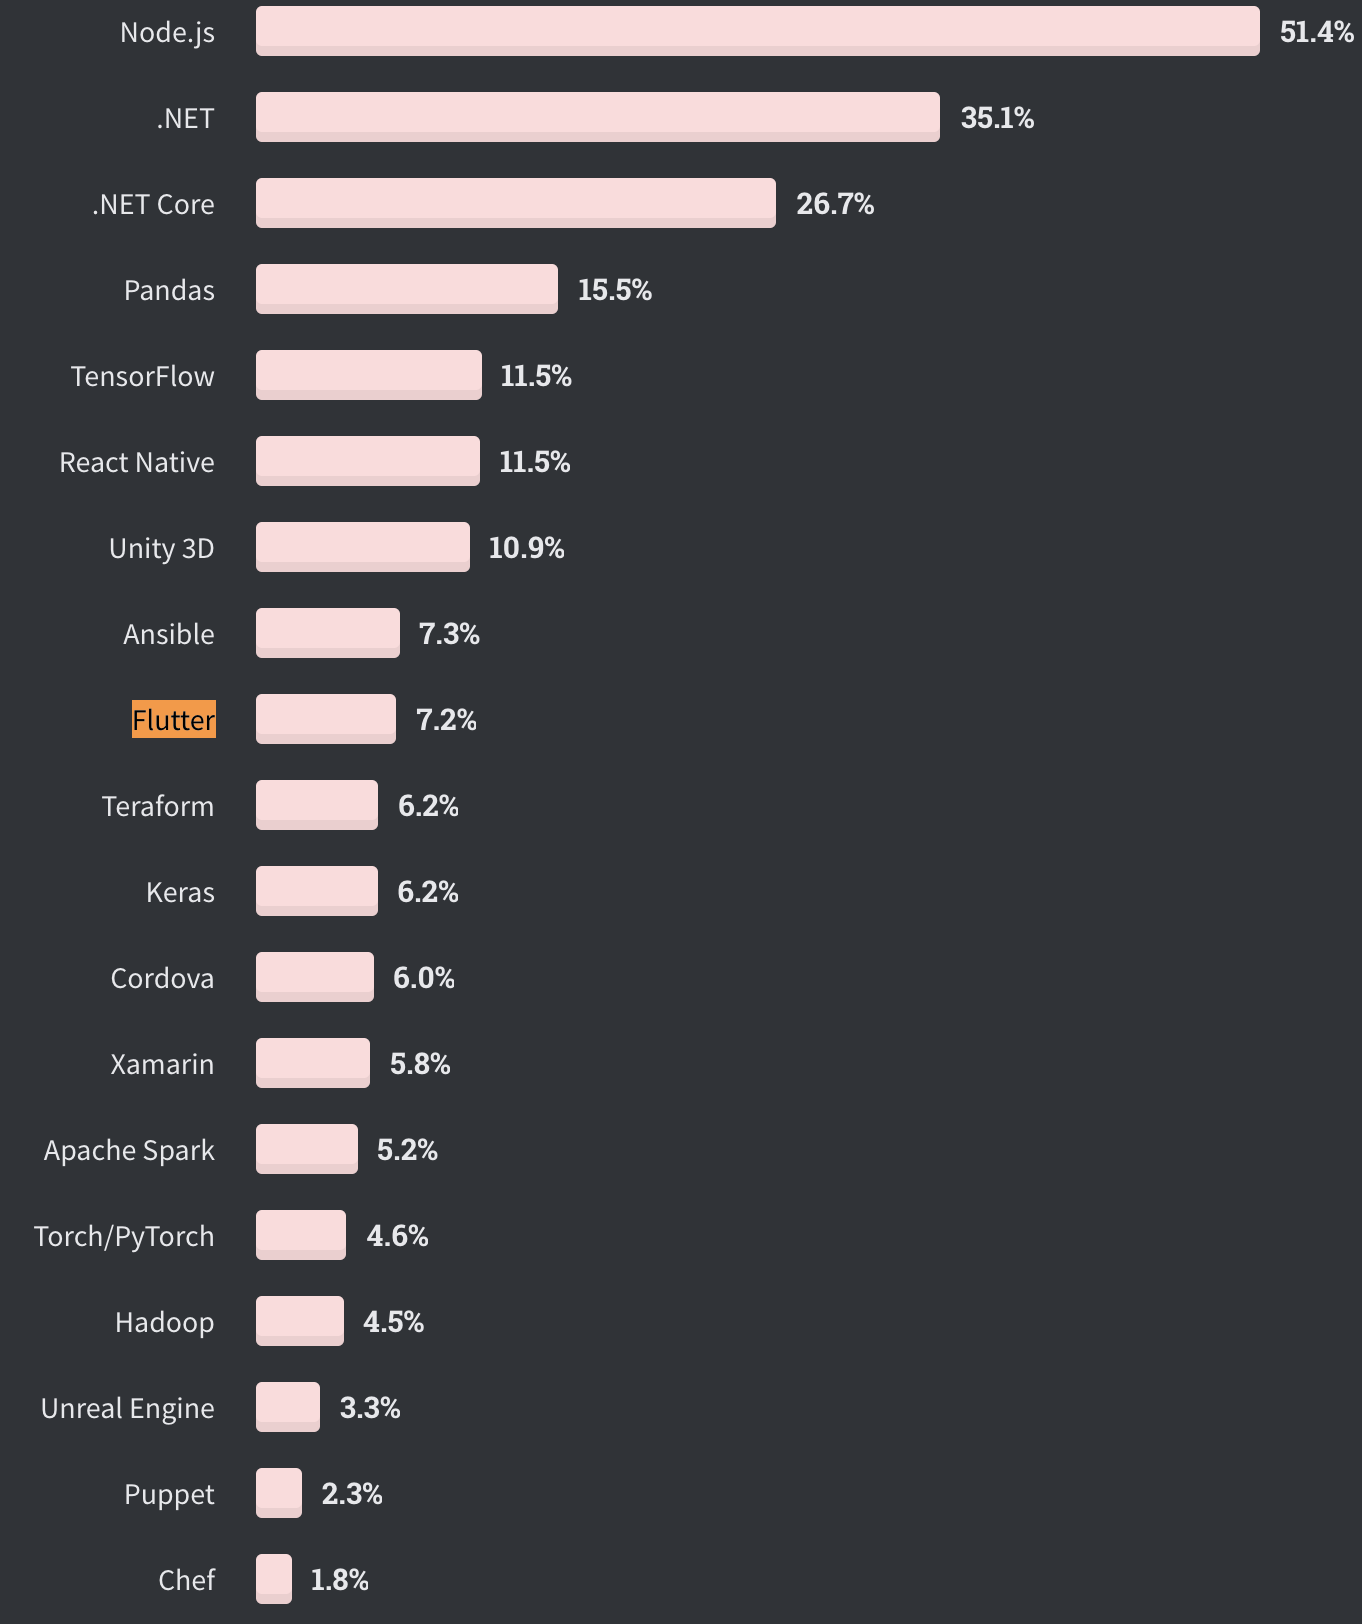
\includegraphics[scale=0.4]{stackoverflow_survey_2020.png}
    \end{center}

    Основна популярність за результатами опитування, яке охопило 40 000 відповідей.
    \cite{stackoverflow_survey_2020}
\end{figure}


\section{Недоліки Flutter}\label{section.1.4}
\begin{enumerate}
    \begin{item}
        Він має обмеження щодо надання інтерфейсу користувача на власних платформах, наприклад, відео на Apple TV або Android TV.
    \end{item}
    \begin{item}
        Функції, що нещодавно додані в рідних системах iOS та Android, природно будуть представлені у Flutter пізніше, ніж у їхніх рідних версіях.
    \end{item}
    \begin{item}
        Незважаючи на те, що Flutter легко вивчити, вам, мабуть, знадобиться певний досвід розробки власних додатків, щоб створити функціональний крос-платформний додаток.
    \end{item}
\end{enumerate}


\section{Переваги React Native}\label{section.1.5}
\begin{enumerate}
    \begin{item}
        Це зрілий фреймворк зі стабільним API, який підтримується Facebook.
    \end{item}
    \begin{item}
        Легко навчитися розробникам React та JavaScript.
        Ви можете скористатися наявними бібліотеками React, інструментами, фреймворками та навчальними посібниками.
        Структура також має велику спільноту розробників.
    \end{item}
    \begin{item}
        Так само, як Flutter, він дозволяє швидко розроблювати додатки iOS, Android та Web зі спільною кодовою базою.
    \end{item}
    \begin{item}
        React Native дозволяє додавати новий код до запущеної програми, що зменшує ризик втрати деяких функціональних можливостей під час повного перезавантаження або відновлення програми.
    \end{item}
\end{enumerate}


\section{Недоліки React Native}\label{section.1.6}
\begin{enumerate}
    \begin{item}
        У ньому все ще бракує певних спеціальних модулів, специфічних для платформи, і для їх створення вам може знадобитися досвід native розробника.
    \end{item}
    \begin{item}
        Навігація не є плавною.
    \end{item}
    \begin{item}
        Міжплатформна розробка може спричинити проблеми з продуктивністю оскільки використовується додатковий рівень інтерпретації коду в runtime середовищі.
    \end{item}
    \begin{item}
        Це не найкращий вибір для програм, які потребують складну анімацію (на приклад ігри).
    \end{item}
\end{enumerate}


\section{Мови програмування}\label{section.1.7}

Flutter використовує мову, що називається Dart.
Це мова, яка має синтаксис, подібний до Java та Javascript.

Простим прикладом коду в Dart буде:
\begin{lstlisting}[style=light, language=Python,label={lst:vectorimg},caption=Dart Hello World]
void main () { 
  print ("Hello World!"); 
}
\end{lstlisting}

React Native використовує Javascript.
React Native побудований поверх React, який побудований на Javascript.
Тому, якщо вам доведеться вивчити React Native, вам знадобляться попередні знання Javascript.

Javascript існує довкола спільноти розробників програмного забезпечення дуже давно, і існує безліч ресурсів, на яких можна навчитися javascript.
Простим прикладом коду в javascript буде:

\begin{lstlisting}[style=light, language=Python,label={lst:vectorimg},caption=Dart Hello World]
  alert("Hello World!");
\end{lstlisting}


\section{Спільнота}\label{section.1.8}

Flutter і Dart були представлені спільноті розробників нещодавно, і порівняно, у неї менша спільнота розробників.
Google витратив багато на розробку Dart, і спільнота продовжує зростати.
Flutter має спільноти на StackOverflow, Slack та багатьох інших платформах.

React Native має більшу спільноту розробників, ніж Flutter, сприяючи його розвитку.
Спільнота Javascript є навіть більшою, ніж спільнота React Native, оскільки вона існує вже дуже давно, і допомогу можна знайти майже скрізь в Інтернеті.
Це, безумовно, пояснює, чому React Native має вищий рівень прийняття в порівнянні з Flutter.
Крім того, підтримка React, React Native та Javascript в Інтернеті є більш доступною.
Є мільйони рядків коду, які є у вільному доступі в Інтернеті, і їх можна просто «зняти» та використовувати у своїх проектах.
На сторінці спільноти React Native на їх офіційному веб-сайті вказані інші платформи, що вміщують їхні спільноти, такі як StackOverflow та Medium.


\section{Віджети інтерфейсу користувача}\label{section.1.9}
Найкраще у Dart - це те, що він постачається з повним набором віджетів інтерфейсу, які можна підняти прямо з коробки та використовувати.
В React Native, набір віджетів інтерфейсу мінімальний, і тому розробникам програмного забезпечення та програмістам доводиться звертатися до сторонніх бібліотек для віджетів інтерфейсу, і іноді їм доведеться створювати власні віджети інтерфейсу.


\section{Порівняння доступних вакансій на ринку Британії}\label{section.1.9}
Розглянемо статистичні дані, щодо популярності платформ на ринку праці.
В якості ринку праці був вибран останій на території Великої Британії, оскільки остання має досить розвиненний ринок IT.
За додаткову метрику розглянемо кількість вакансій доступних за остатні 6 місяців.

Отже вакансій доступних для React Native розробників 877, де 908 було за той самий період в 2020 і 750 за 2019 \cite{react_native_jobs}.
Вакансій на Flutter меньше всього 113 за 2021, 49 за 2020 та 12 за 2019 \cite{flutter_jobs}.
Враховуючи ці дані можна зробити висновок, що React Native показує більшу зацікавленість ринку праці.
Однак, в захист Flutter можна додати, що за остатній рік в рейтингу вакансій Flutter піднявся на 309 пунктів \cite{flutter_jobs}, коли React Native на 165 \cite{react_native_jobs}.

Нажаль схожої статистики по Kotlin Mutliplatform не вдалося точно виявити.
Загальна тенденція вакансій по Kotlin, як мові програмування показує нам 917 за 2021, 1 196 за 2020 та 644 за 2019 роки \cite{kotlin_jobs}.

Цікавим спостереженєм є медіана зарплат де Kotlin розробника пропонують £70,000\cite{kotlin_jobs}, React Native £60,000\cite{react_native_jobs} та Flutter £52,500\cite{flutter_jobs}.
Таку тенденцію можно пояснити широкопрофільним застосуванням Kotlin, як в розробці Backend так і Frontend клієнтів.


\section{Декларативність системи React}
\label{section.1.10}

React \textbf{декларативний} та спрощує створення інтерактивних інтерфейсів.
Вам потрібно лише описати, як різні частини інтерфейсу виглядають у кожному стані вашого додатку і React ефективно оновить та відрендерить лише потрібні компоненти.
Декларативні інтерфейси роблять наш код більш передбачуваним і його набагато легше налагоджувати.

React Native \textbf{заснований на інкапсульованих компонентах}, які керують власним станом, і з них будують складні інтерфейси.
Оскільки логіка компонентів написана на JavaScript, замість шаблонів, ми з легкістю можемo передавати складні дані у додатку і зберігати стан окремо від DOM.

Розглянемо оголошення змінної:
\begin{lstlisting}[style=light, language=Python,label={lst:jsx_hello},caption=JSX Hello World]
const element = <h1>Hello, world!</h1>;
\end{lstlisting}

Цей дивний синтаксис тегів не є ні рядком, ні HTML.

Він має назву \textbf{JSX}, і це розширення синтаксису для JavaScript.
Його використовує React, щоб описати інтерфейс користувача.
JSX може нагадувати мову шаблонів, але з усіма перевагами JavaScript.

React використовує той факт, що логіка виводу пов’язана з іншою логікою інтерфейсу користувача: як обробляються події, як змінюється стан з часом і як дані готуються для рендерингу.

Замість того, щоб штучно відокремити технології, розмістивши розмітку і логіку в окремих файлах, React розділяє відповідальність між вільно зв’язаними одиницями, що містять обидві технології і називаються "компонентами".
React не вимагає використання JSX, але більшість людей цінують його за візуальну допомогу при роботі з інтерфейсом користувача в коді JavaScript.
Він також дозволяє React показати зрозуміліші повідомлення про помилки та попередження.


\section{React та система побудування Expo}
\label{section.1.11}
React Native пропонує два різних способи побудування проекту \textbf{«керований»} та \textbf{«простий»} робочими процесами.
\begin{itemize}
    \begin{item}
        За допомогою \textbf{керованого} робочого процесу ви пишете лише інструменти та служби JavaScript / TypeScript та Expo, які піклуються про все інше.
    \end{item}
    \begin{item}
        У \textbf{простому} робочому процесі ви маєте повний контроль над кожним аспектом власного проекту, а інструменти та послуги Expo трохи більш обмежені.
    \end{item}
\end{itemize}

В обох випадках використовується екосистема інструментів, що спрощують процес пободування проекту, ховаючи деталі та називається Expo.
Expo - платформа для універсальних додатків React, набір інструментів та служб, побудованих навколо React Native та власних платформ, які допомагають вам розробляти, будувати, розгортати та швидко переглядати iOS, Android та веб-додатки з тієї самої кодової бази JavaScript / TypeScript.\cite{expo_doc}


\section{Запити до мережі. Fetch API}
\label{section.1.12}
React Native надає API Fetch для ваших мережевих потреб.
API Fetch забезпечує інтерфейс для отримання ресурсів (у тому числі по всій мережі).
Буде здаватися звичним кожному, хто використовував XMLHttpRequest, але новий API забезпечує більш потужний та гнучкий набір функцій.
Fetch забезпечує загальне визначення Requestі Responseоб'єктів (та інших речей, пов'язаних із мережевими запитами).
Це дозволить їх використовувати там, де вони потрібні в майбутньому.

Fetch API залежить від Promise.
Promise або "обіцянка" - це проксі для значення, яке не обов'язково відомо при створенні об'єкту.\cite{promise_doc}
Інакше кажучи, це API обгортка, яка задає контракт згідно которого promise(обіцянка) може знаходитись в одному зі станів:
A Promise знаходиться в одному з таких станів:
\begin{itemize}
    \begin{item}
        \textbf{в очікуванні(peding)}: початковий стан, ні виконаний, ні відхилений.
    \end{item}
    \begin{item}
        \textbf{виконано(fulfilled)} : це означає, що операція була успішно завершена.
    \end{item}
    \begin{item}
        \textbf{відхилено(rejected)} : означає, що операція не вдалася.
    \end{item}
\end{itemize}

Прикладом коду, котрий виконує запит та отримує відповідь в форматі JSON можна знайти в додатку \ref{lst:rn_network}.


\section{Realm React Native}
\label{section.1.13}
В випадку вибору бази даних треба розглянути наступні фактори:
\begin{itemize}
    \begin{item}
        \textbf{Технологія:} з відкритим кодом чи власністю?
    \end{item}
    \begin{item}
        \textbf{Архітектура:} SQL або NoSQL?s
    \end{item}
    \begin{item}
        \textbf{Масштабованість:} чи ви будете самостійно розміщувати або скористаєтесь масштабованою послугою?
    \end{item}
\end{itemize}

Ринок надає можливість використання таких рішень як:

\begin{longtable}[c]{|l|l|l|}
    \caption{Порівняння Баз Даниx React Native}
    \label{tab:rn_db_comparison} \\
    \hline
    & Сирцевий код  & Тип реаліаційної БД \\ \hline
    \endhead
%
    Back4app        & Відкритий     & SQL, NoSQL          \\ \hline
    Cloud Firestore & Пропрієтарний & NoSQL               \\ \hline
    DigitalOcean    & Відкритий     & SQL                 \\ \hline
    AWS RDS         & Відкритий     & SQL                 \\ \hline
    Realm           & Відкритий     & NoSQL               \\ \hline
\end{longtable}

Під час роботи над тестовим продуктом було зроблене рішення використати Realm.
Рішення базувалося скоріше на потребах швидкого та простого в інтеграції рішення.
Як наведено в додатку \ref{lst:rn_realm}  конфігурація в цілому є дуже проста (також див. \ref{fig:rn_realm}).

Спочатку ми описуємо схему бази даних. В даному випадку одна таблиця.
Створюємо об'єкт конфігурації, котрий буде використаний, щоби відкрити підключення до бази даних.
Передавши конфігурацію ми отримаємо відкрите підключення до бази даних та робимо запит до таблиці.
Запит повертає нам результат зі збереженими даним з котрих ми робимо копію кожного об\'єкту.
Особливість Realm об\'єктів полягає в тому, що вони є вікном до курсору в таблиці.
Щоби уникнути випадкових змін в таблиці ми спеціально робимо копію, яка є "чистим" об\'єктом від\'єднаним від БД.

\begin{figure}
    \label{fig:rn_realm}
    \begin{center}
        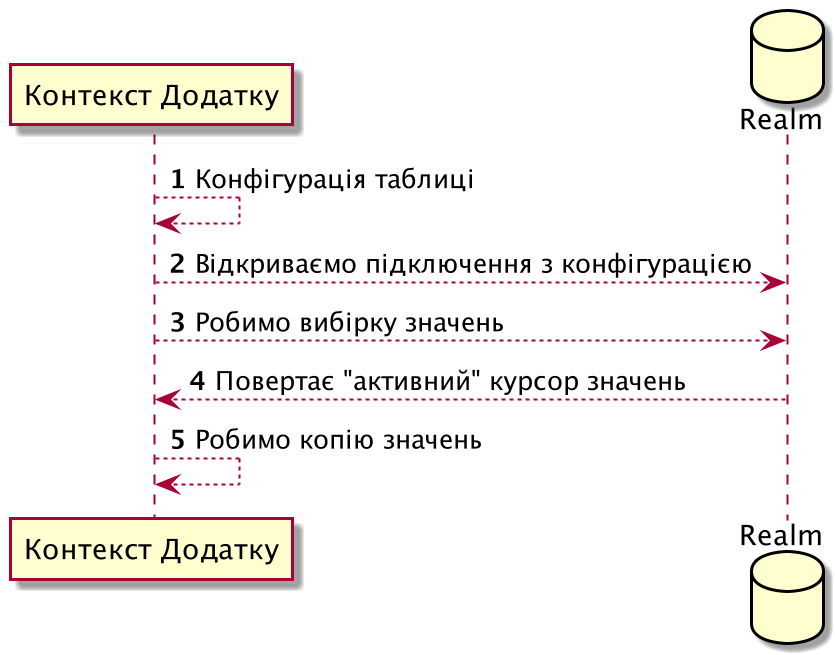
\includegraphics[scale=0.4]{rn_realm.png}
    \end{center}

    Взаємодія React Native додатку з БД
\end{figure}


\section{React Native та управління станом}
\label{section.1.14}

Даний підхід дозволяє швидко і в простий спосіб сконфігурувати стан нашого компоненту.
Хоч це і звучить просто нажаль, в більш складних компонентах з великою кількістю взаємодій з користувачем такий підхід призведе до високої зв'язаності коду.
В свою чергу ми отримаємо складний до зрозуміння сирцевий код і нестабільне рішення з великою кількістю помилок.
Для рішення цієї проблеми можна застосувати архітектуру Redux.

Redux - передбачуваний контейнер стану для Javscript додатків Apps (див. на \ref{fig:rn_realm}))..
Redux допомагає писати програми, які поводяться послідовно , працюють у різних середовищах (клієнтських, серверних та власних) і легкі для перевірки. \cite{redux_home_page}
Централізація стану та логіки вашого додатка забезпечує потужні можливості, такі як скасування / повтор , стійкість стану та багато іншого. \cite{redux_home_page}

\begin{center}
    \begin{figure}
        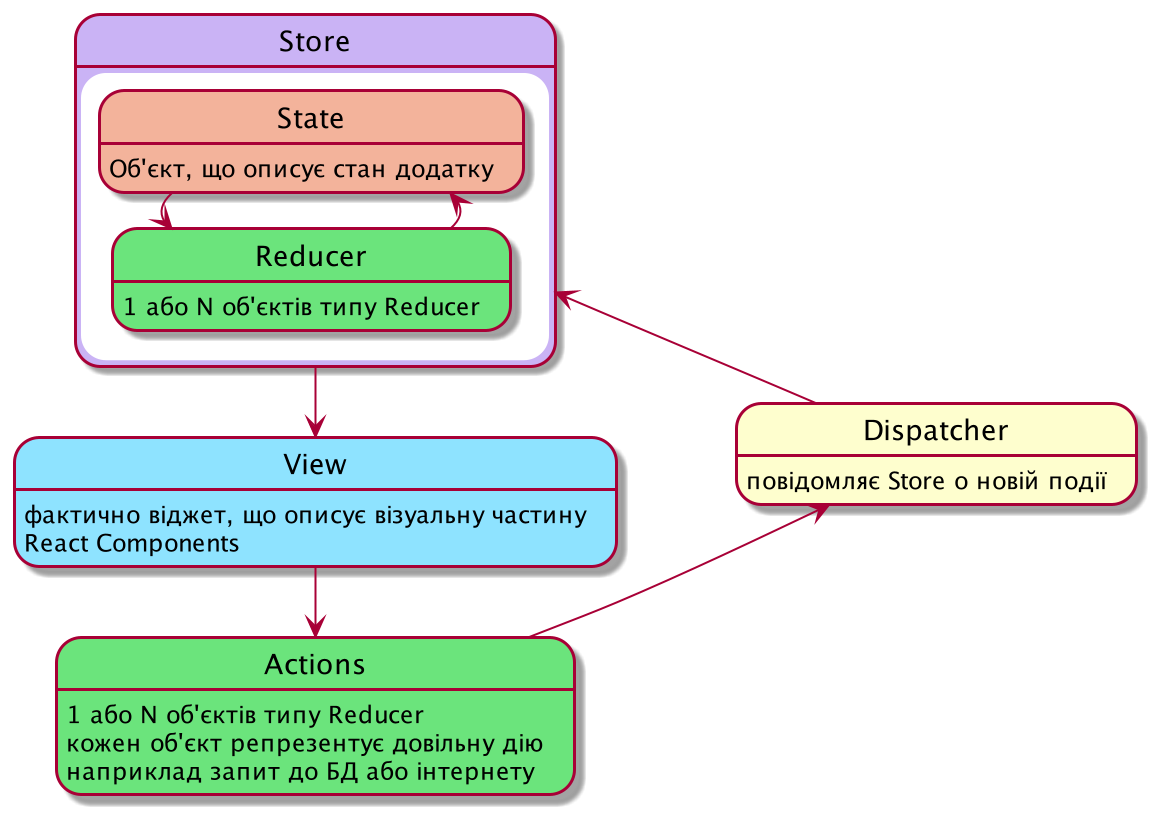
\includegraphics[scale=0.33]{redux.png}
        \caption{Схема Redux}
        \label{fig:rn_redux}
    \end{figure}
\end{center}


\section{Тестування в React Native}
\label{section.1.15}
У міру розширення вашої кодової бази невеликі помилки та крайні випадки, на які ви не очікуєте, можуть перетворюватися на більші збої.
Помилки призводять до поганого досвіду для користувачів і, зрештою, до втрат бізнесу.
Одним із способів полібшити якість сирцевого коду є написання тестів.

Одним з найкращих способів виправити помилку в коді є написання тесту, який виявляє її.
Потім, коли ви виправляєте помилку і повторно запускаєте тест, якщо він проходить, це означає, що помилка виправлена, і ніколи повторно не буде впроваджена в сирцевий код проекту.

Тести також можуть служити документацією для нових людей, які приєднуються до вашої команди.
Людям, які ніколи раніше не бачили кодової бази, аналіз тестів може допомогти зрозуміти, як працює існуючий код.
Нарешті, але не менш важливим є те, що більш автоматизоване тестування означає менше часу, проведеного за допомогою ручного контролю якості, звільняючи цінний час.

За замовчуванням React Native постачається з тестовою структурою Jest. \cite{jest_home_page}

\begin{lstlisting}[style=light, language=Python,label={lst:rn_jest_test},caption=Jest Unit Test]
  it('given 2 +2 returns 4', () => {
    expect(2 + 2).toBe('red');
  });
\end{lstlisting}

Jest дозволяє групувати тести з уживанням функцій "describe"(опис).
Підтримує хуки для ініціалізації стану "beforeEach"(перед кожним) та "beforeAll"(після всіх).

Unit test(єдносткові тести) допомагають протестувати тільки бізнес логіку.
Для тестування UI компонентів застосовується компонентне тестування.
Навіть якщо логіка вашого додатка має високий рівень охоплення тестуванням і є правильною,
без тестування компонентів ви все одно можете доставити непрацюючий інтерфейс для своїх користувачів.

Під час тестування компонентів React можна перевірити дві речі:

\begin{itemize}
    \begin{item}
        \textbf{Взаємодію:} для забезпечення належної поведінки компонента під час взаємодії з ним користувачем (наприклад, коли користувач натискає кнопку)
    \end{item}
    \begin{item}
        \textbf{Рендеринг:} щоб переконатися, що вихідний вигляд компонента, який використовує React, правильний (наприклад, зовнішній вигляд кнопки та розміщення її в інтерфейсі)
    \end{item}
\end{itemize}

Однак требу мати на увазі, що тестування компонентів - це лише тести JavaScript, що виконуються у середовищі Node.js.
Вони не беруть до уваги будь-який iOS, Android або інший код платформи, який підтримує компоненти React Native.
Звідси випливає, що вони не можуть надати вам 100\% впевненості, що все працює.
Якщо в коді платформи iOS або Android є помилка, вони її не знайдуть.

Останій клас тестів - це ті, що дозволяють протестувати в наскрізний спосіб наш додаток (далі E2E - End to End).
Це робиться шляхом запуску тестів на фінальній зборці додатку виконаному в середовищі Android або iOS.
У тестах E2E ви більше не думаєте про компоненти React, React Native API, Redux чи будь-яку бізнес-логіку.

Тести E2E дають вам максимально можливу впевненість у тому, що частина вашого додатка працює.
Однак в випадку E2E ми мусимо враховувати наступні компроміси.

\begin{itemize}
    \item їх написання займає більше часу порівняно з іншими типами тестів
    \item вони працюють повільніше
    \item вони більш нестабільні "flakky" ("flakky"  - це тест, який випадково проходить і не проходить без будь-яких змін в коді)
\end{itemize}

Доступно кілька інструментів тестування E2E.
\begin{itemize}
    \item у спільноті React Native Detox є популярним фреймворком, оскільки він спеціально підходить для додатків React Native.\cite{detox_home_page}
    \item ще однією популярною бібліотекою для iOS та Android додатків є Appium.\cite{appium_home_page}
\end{itemize}

\section{FLutter порівнняня віджетів з/без стану}
\label{section.1.16}
Однією з основних тем, яка супроводжує вас під час використання Flutter, є те, що на 80\% розробки це потужне використання віджетів.

Віджети Flutter побудовані з використанням сучасного фреймворку, який черпає натхнення у React \cite{flutter_widgets_intro}.
Основна ідея полягає в тому, що ви створюєте свій інтерфейс з віджетів.
Віджети описують, як повинен виглядати їхній вигляд, враховуючи їх поточну конфігурацію та стан.
Коли стан віджета змінюється, віджет відновлює свій опис, при цьому фреймфорк порівнює новий стан з попереднім,
визначає мінімальні зміни, та оновлює дерево візуалізації, таким чином, переходячи з одного стану в наступний.

Головна структура будь-якого Flutter додатку будується на основі віджетів.
Згідно з специфікацією Dart першочергове, що ми робимо це імпортоування компенентів за допомогою конструкції \textbf{import}.
Наступними кроками буде ініціалізація в \textbf{main()} функції дерева віджеті \textbf{WidgetsFlutterBinding.ensureInitialized() та
виклик функції \textbf{runApp()}, що прив'язує визначене нами дерево віджетів.

Далі ми наводимо сирцевий код, що описує логіку ініціалізації додатку та визначає головний віджет додатку. \ref{lst:flutter_app_widget}
Як ми бачимо з наведеного сирцевого коду, по суті, розробка в Flutter подібна до гри з матрьошкою,
де ми вкладаємо один віджет в настуапний поступово додаючи складність до розвязання.

Треба звернути увагу, що головний віджет не має стану і тим самим визначає, що кореневий віджет буде не змінним
під час перерахування дерева після зміни стану в інших шарах додатку.

Тепер ознайомившись з прикладом віджету без стану, слід навести протилежність, а саме StateFullWidget(зі станом).
Ми зробимо це на прикладі списку котрий відображає додаток. \ref{lst:flutter_app_widget}

Головне, що требу розуміти в випадку віджетів зі станом це те, що зміна стану приводить до перемалювання віджету.
Оскільки один віджет може повертати довільно складне дерево віджетів змінивши стан голови гілки призведе до змін
ланки віджетів, що наслідує наш віджет зі станом.

\section{Система побудування з використанням Flutter CLI}
\label{section.1.17}
Flutter CLI - інструмент командного рядка котрий дозволяє створити, виконати, зібрати сирцевий код проектів фреймфорку Flutter.

\begin{lstlisting}[style=light, language=Python,label={lst:flutter_cli_create},caption=Flutter Create Project]
flutter create my_app
cd my_app
flutter analyze
flutter test
flutter run lib/main.dart
\end{lstlisting}

Як видно в лістингу \ref{lst:flutter_cli_create} ми виконуємо команду, що створює, перевіряє, запускає тести та відтворює фактично код додатку.

Додатково набір інсрументів дозволяє завантажити, сконфігурувати та під'єднати транзитивні залежності проекту \ref{lst:flutter_pub}.
\begin{lstlisting}[style=light, language=Python,label={lst:flutter_pub},caption=Flutter Dependency Resolution]
flutter pub get
flutter pub outdated
flutter pub upgrade
\end{lstlisting}

Повний список залежностей можна знайти на офіційній веб сторінці \cite{flutter_cli}.

\section{Flutter та пакет http.dart}
\label{section.1.18}
Отримання даних з Інтернету необхідно для більшості програм.
На щастя, Dart і Flutter надають інструменти, такі як httpпакет, для цього виду робіт.

Цей пакет містить набір функцій та класів високого рівня, що полегшують споживання ресурсів HTTP.
http.dart підтримує мобільну, настільну та браузерні платформи.

Використання функцій верхнього рівня дозволяє робити окремі HTTP-запити.
Якщо є потреба робити кілька запитів на один і той же сервер, тоді зручніше всього тримати відкритим постійне з’єднання,
використовуючи клієнт, а не одноразові запити.

\begin{lstlisting}[style=light, language=Python,label={lst:flutter_pub},caption=Flutter Dependency Resolution]
import 'package:http/http.dart' as http;
var client = http.Client();
try {
  var uriResponse = await client.post(Uri.parse('https://example.com/whatsit/create'),
      body: {'name': 'doodle', 'color': 'blue'});
  print(await client.get(uriResponse.bodyFields['uri']));
} finally {
  client.close();
}
\end{lstlisting}

\section{Flutter та пакет sqflite}
\label{section.2.4}
SQFlite - це порт SQLite драйверу для платформ написаних на Dart, яке підтримує iOS, Android та MacOS.

До можливостей sqflite можна віднести:

\begin{itemize}
    \item Підтримка транзакцій та пакетів.
    \item Помічники для вставки / запиту / оновлення / видалення запитів.
    \item Операції до БД, виконуються у фоновому потоці на iOS та Android.
    \item Підтримка Linux / Windows / DartVM за допомогою sqflite_common_ffi.
\end{itemize}
